\documentclass[a4paper,10pt]{article}
% disable annoying warning
% from time to time try to delete this as there might be a fix deployed in the font package
% https://github.com/tectonic-typesetting/tectonic/issues/924
\newcount\XeTeXtracingfonts

\usepackage[utf8]{inputenc}

\usepackage{hyperref}
\usepackage{graphicx}

% with the default options it reduces the page margins already
\usepackage{geometry}

% glossary {{{
\usepackage[acronym,automake]{glossaries}
\makeglossaries

% \newglossaryentry{WAUT}
% {
%     name=WAUT,
%     description={Web Application Under Test}
% }
\newacronym{waut}{WAUT}{Web Application Under Test}
\newacronym{spa}{SPA}{Single Page Application}
\newacronym{ssg}{SSG}{Static Site Generator}
% }}}

\title{Run-time verification of web applications}
\author{Roberto Tonino}
\date{2025-03-21}

% cool font {{{
% \usepackage[utf8]{inputenc}
\usepackage{libertine}
% \usepackage{libertinust1math}
% \usepackage[T1]{fontenc}
% % }}}

% biblatex {{{
\usepackage{biblatex}
\addbibresource{report.bib}
% }}}

\usepackage{ifthen}

\newcommand{\tuple}[1]{\mbox{$\langle$#1$\rangle$}}
% \newcommand{\reqmulti}[1]{\mbox{$\langle r_{#1}$,$l_{#1}$,$t_{#1}\rangle$}}
\newcommand{\reqmulti}[1][]{
  \ifthenelse{\equal{#1}{}} {\mbox{$\langle r$,$l$,$t\rangle$}}
  {\mbox{$\langle r_{#1}$,$l_{#1}$,$t_{#1}\rangle$}}
}

\newcommand{\res}[1][]{
  \ifthenelse{\equal{#1}{}}{\mbox{$\langle u$, $c$, $I$, $L$, $V\rangle$}}
  {\mbox{$\langle u_{#1}$, $c_{#1}$, $I_{#1}$, $L_{#1}$, $V_{#1}\rangle$}}
}
\newcommand{\resmulti}[1][]{
  \ifthenelse{\equal{#1}{}}{\mbox{$\langle u$, $c$, $I$, $F$, $L$, $V\rangle$}}
  {\mbox{$\langle u_{#1}$, $c_{#1}$, $I_{#1}$, $F_{#1}$, $L_{#1}$, $V_{#1}\rangle$}}
}

% theorem {{{
\usepackage{amsthm}

\theoremstyle{plain} % default
\newtheorem{thm}{Theorem}[section]
\newtheorem{lem}[thm]{Lemma}
\newtheorem{proposition}[thm]{Proposition}
\newtheorem*{cor}{Corollary}

\theoremstyle{definition}
\newtheorem{example}{Example}[section]
\newtheorem{definition}{Definition}[section]
\newtheorem{procedure}{Procedure}

\theoremstyle{remark}
\newtheorem{rmrk}{Remark}[section]
\newtheorem{note}{Note}[section]

\usepackage[capitalize,nameinlink]{cleveref} % from https://tex.stackexchange.com/questions/187388/amsthm-with-shared-counters-messes-up-autoref-references
% Customize cref names
% Generated by Claude
\crefname{example}{Example}{Examples}
\crefname{rmrk}{Remark}{Remarks}
\crefname{lem}{Lemma}{Lemmas}
\crefname{procedure}{Procedure}{Procedures}

% }}}

\begin{document}

\maketitle

\tableofcontents

\clearpage

\section{Introduction}

This report summarizes the paper \citetitle{Haydar2013}. The authors present a solution that uses finite automata, LTL and the model checker Spin to formally verify properties on web applications.

The paper begins explaining how to build the automata that are used to model the behaviour of the user in a web application. After that, the authors focus on LTL, presenting a new operator that allows formula writers to define an LTL formula scoped to a subset of states. Eventually, the authors conclude the paper showing empirical results, together with a prototype of a tool to apply all the steps described in the paper.

\section{Definitions}

Some definitions are now presented, which will help the reader understand the technical jargon discussed in the paper:

\begin{itemize}
  \item \textit{\gls{waut}}: the web application taken in consideration in a particular definition, discussion, etc...
  \item \textit{request}: string $l$ that represents a web request performed by a \gls{waut}
  \item \textit{response}: tuple \res which represents the response that the web server sent to the \gls{waut}
    \begin{itemize}
      \item $u = l$
      \item $c$ represents the status code of the response \cite{Fielding2022}
      \item $I =$ ``target'' attribute of the forms contained in the response
      \item $L =$ URLs of the links contained in the response
      \item $V =$\ <$v_1,\dots,v_k$> vector where $v_i$ is the valuation of the page attribute $i$
    \end{itemize}
  \item \textit{browsing session}: recorded sequence of request-response exchanges that a user performs when visiting a \gls{waut}
  \item \textit{local browsing session}: recorded sequence of request-response exchanges that a user performs in a single browser window or frame
\end{itemize}

\section{Automata}

In order to represent the behaviour of a user in a web application, the authors propose a \emph{communicating-automata}-based model of the \gls{waut}. An automaton represents the ``journey'' that a user takes when utilizing the \gls{waut}: this journey is identified by the links that the user clicks or the forms that they submit, and the pages that are loaded subsequentially. For an easier understanding, the authors present an incremental approach to the communicating-automata model. A \textit{single-display} application model is first proposed, then to be followed by a \textit{multi-display} application model.

\subsection{Single-display applications model}
\label{single-display-applications}

% maybe add a part where we define request, response ecc...? Yes and no, I don't want it to make a copy of the original paper
% at least the tuple has to be defined

The automaton that represents a single-display application is built as follows.

\begin{procedure}
  \label{browsing-session-to-automaton}
  Convert a browsing session of a single-display application into an automaton.

  \begin{enumerate}
    \item the inactive state $s_0 = \res[0]$ is defined;
    \item the set of states is defined by the set of \emph{responses}, a response being \res[i]
      \begin{enumerate}
        \item when only the links in two responses are different, the responses are mapped to the same state. The authors provide a proof that this compression does not alter the recorded behaviour of the \gls{waut};
      \end{enumerate}
    \item the alphabet is built from the union of the requests ($Req$), the URIs associated with links in the observed responses ($\Gamma$), and the actions that correspond to the unexplored forms in the observed responses $\Delta$. $\Sigma=Req\cup\Gamma\cup\Delta$;
    \item there is a transition $(s_i,l_{i+1},s_{i+1})$ from state $s_i$ to state $s_{i+1}$ if there is a link or a form action that goes the page represented by $s_i$ to the page represented by $s_{i+1}$;
    \item requests corresponding to explored forms or links define a transition that goes from the state where the request occurs to the state mapped to the response;
    \item for each unexplored link $l \in L_i$ or form $a \in I_i$, the automaton has a transition from the state representing the page \res[i] to a so-called \textit{trap} state $t \in T$.
  \end{enumerate}
\end{procedure}

The construction allows to define \emph{deduced} links: they are links that are \textbf{not} visited during the browsing session, but are contained in one or more of the responses of the browsing session. Deduced links extend the automaton, making it a little more complete, enhancing property verification and improving reachability of certain states.

In \cref{fig:example-session-automaton} it is possible to see an example of a constructed session automaton. The links ``URL1'', ``URL2'', and ``URL3'' are unexplored links which transition to the trap state. The transitions from $s_2$ to $s_1$, from $s_3$ to $s_2$, and from $s_4$ to $s_1$ represent deduced links. Notice that deduced links are undistinguishable from regular links in the automaton representation.

\begin{figure}[h]
  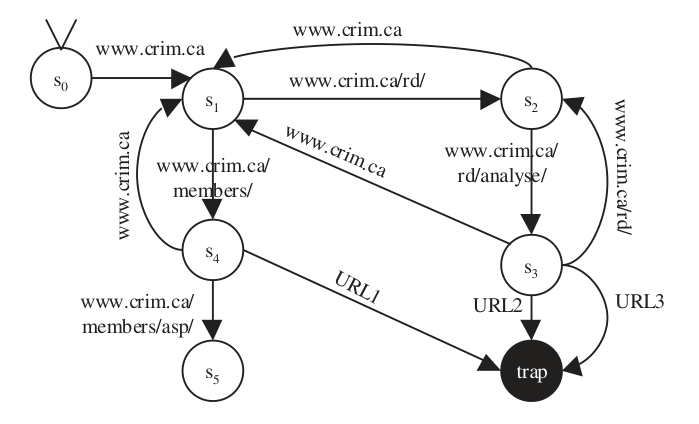
\includegraphics[width=\textwidth]{img/session_automaton_example.png}
  \caption{Example of a session automaton.}
  \label{fig:example-session-automaton}
\end{figure}

\subsection{Multi-display applications}

The model presented in \cref{single-display-applications} is extended to handle multi-window and multi-frame applications. Such applications intrinsically possess concurrency because of how browsers load them: in the case of a web page with several frames, it is not possible to know in advance what will be the loading order of the pages. The authors note how it is theoretically possible to represent multi-display as single-display applications, but it is discouraged because it is cumbersome to represent multiple, parallel behaviours in a single automaton. Some of the definitions are extended from the ones of single-display applications:

\begin{itemize}
  \item \textit{response:} \resmulti with $F$ being a set of frames in the page. The target $t$ is defined; if no target is present $t = \varepsilon$. Additional changes are:
    \begin{itemize}
      \item \tuple{$i$, $t$} $\in L$
      \item \tuple{$a$, $t$} $\in I$
      \item \tuple{$f$,$b$} $\in F$
    \end{itemize}
  \item the requests are now made of the link as before, with the addition of the referer (link from which the request started) and the target (TODO expand with formalisms)
\end{itemize}

The procedure for building a single-display automaton is extended to build a communicating automata model.

\begin{procedure}
  Convert a browsing session of a multi-display application into a communicating automata model.

  \begin{enumerate}
    \item a browsing session is split into a local browsing session $(RRS_1,\dots,RRS_k)$, one for each window and frame;
    \item convert each local browsing session into an automaton (TODO add formalisms);
      \begin{enumerate}
        \item use \cref{browsing-session-to-automaton} to convert a $RRS$ to an automaton;
        \item the alphabet is extended with the source pages of the frames (src attribute)
        \item the case in which the user clicks on a link or submits a form while a frame is loading is handled by adding a transition from each state of the local automaton to the response state
        \item each unexplored link is mapped to a loop in the state it targets (self-loop)
      \end{enumerate}
    \item create the communicating automata via the \textit{parallel composition operator}, denoted $A_1\mid\mid A_2$. The compositions of multiple automata is denoted $A_1\mid\mid\dots\mid\mid A_k$
  \end{enumerate}
\end{procedure}

A detailed explanation is presented in \cite{Haydar2004}.

\section{Extension of the automata model}

In the communicating automata model described above, it is possible to characterize \textit{transient} and \textit{stable} states. Transient states represent situations where a multi-frame page is loaded, and the browser performs the requests for the frames in that page \textbf{without user intervention}.

The authors propose an \textit{extended automata model} by adding a context variable to each state of each automaton. The context variable represents the number of frames that have to be loaded when in a certain state. If the context variable equals 0, the state is denoted stable, i.e. there are no more frames to load. Otherwise, the state is denoted transient.

In \cref{fig:example-communicating-automata} an example of communicating automata is presented. The automata are not in their extended version, but it is possible to denote the transient and stable states already. The transient states are all the states that have an outgoing transition $f_i$, i.e. a transition that represents a frame loaded by the browser without user intevention. The stable states are therefore $(s_0,u_0,w_0)$, $(s_1,u_1,w_1)$, $(s_1,u_2,w_1)$, $(s_2,u_0,w_0)$.

\begin{figure}[h]
  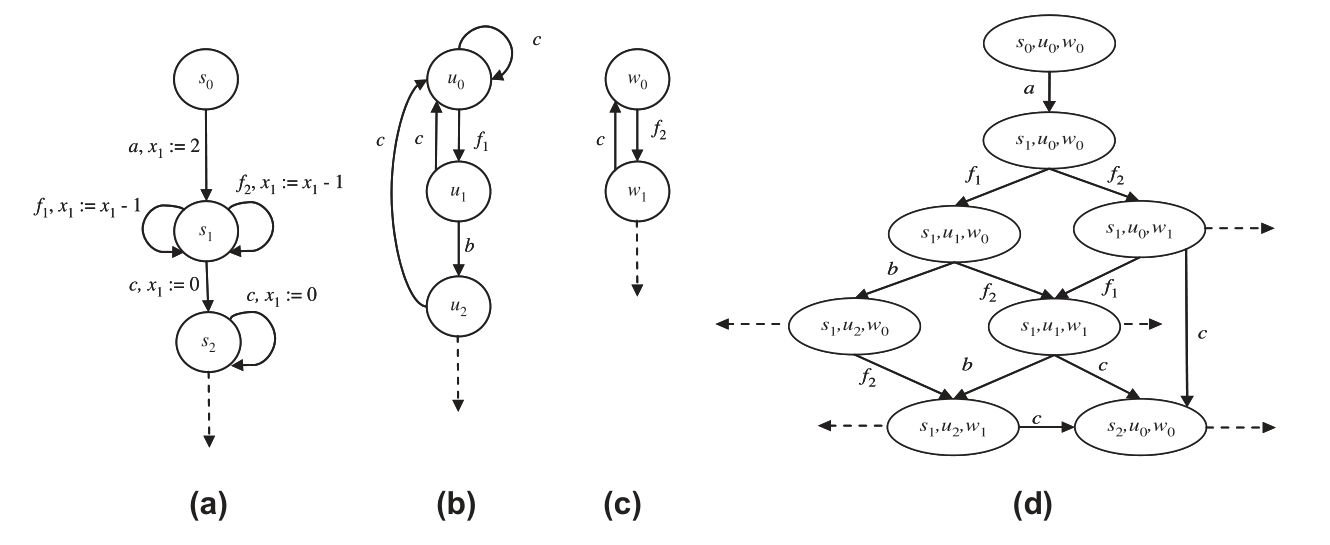
\includegraphics[width=\textwidth]{img/communicating_automata_example.png}
  \caption{Example of communicating automata.}
  \label{fig:example-communicating-automata}
\end{figure}

Each component automaton gets a context variable in each state. When all the component automata are in a state where the context variable is equal to 0, then the global state is considered stable.

\subsection{Extended single-display automaton}

The definition of an Extended Automaton for single-display applications follows:

\begin{procedure}
  \label{extended-single-automaton}
  \begin{enumerate}
    \item the states, alphabet and initial state are unchanged;
    \item $x_i$ is the context variable, $x_{0i}$ is the context variable's initial state;
    \item either
      \begin{enumerate}
        \item if the current state has a loop and $x_i$ is in the designated set of transitions (TODO rephrase, not clear), then decrement the value of $x_i$ by 1;
        \item otherwise set $x_i$ to the number of frames;
      \end{enumerate}
  \end{enumerate}
\end{procedure}

The designated set of transitions $\Sigma^d_i$ is the set of those transitions who cause the automaton to pass through a transient state. In the case of browser sessions, the elements belonging to this set are the \textbf{browser triggered events}.

\subsection{Extended multi-display automaton}

The definition of a \textit{communicating extended automata} model follows:

\begin{enumerate}
  \item build the single-display automata;
  \item apply \cref{extended-single-automaton} to get extended automata;
  \item the set of designated events $\Sigma^d_i$ is the set of frames of the browsing session;
  \item $x_i$ is initially set to 0;
  \item at each state, $x_i$ is assigned the number of frames that have to be loaded by the browser, or it is decremented;
  \item each automaton is unfolded; % TODO rephrase, unclear
  \item the unfolded automata are composed using the composition operator.
\end{enumerate}

The communicating extended automata model built as such is called stable if all its $x_i$ variables are set to 0. Otherwise, it is called transient.

\section{LTL and the In operator}

To ease the definition of properties in a setting with automata possessing transient and stable states, the authors introduce new operators to increase the succintness of LTL. The operators allow to specify LTL properties over a subset of the state space offered by the system in consideration. For example, operators can be used to specify properties that hold only on the main page, or only in a subset of the pages of the application.

Over propositional logic expressions, the $\mathcal{\Im}$-scope operator is introduced. The authors re-define LTL's $\neg$, $\land$, $\lor$ U, X, F, and G operators to use $\mathcal{\Im}$ scopes, defining $\neg_{\mathcal{\Im}}$, $\land_{\mathcal{\Im}}$, $\lor_{\mathcal{\Im}}$, $U_{\mathcal{\Im}}$, $X_{\mathcal{\Im}}$, $F_{\mathcal{\Im}}$, and $G_{\mathcal{\Im}}$. The scope is in itself a logical formula. A formula that is satisifed in a $\Im$ scope is not said to be satisfied outside of the scope.

Over logical formulas, instead, the \textbf{\texttt{In}} operator is introduced, which makes use of the $\mathcal{\Im}$-scope operator. The full specification is detailed in \cite{Haydar2005}.

An example of a simplication allowed by the \textbf{\texttt{In}} operator is the following.

\begin{example}
  $$
  G(((\neg Home\land\neg Shopping) \rightarrow (Promotions = 0))\land ((Home\land Shopping) \rightarrow (Promotions \leq 2)))
  $$
\end{example}

\begin{example}
  \label{example:in-operator-simple}
  $$
  G(((Promotions \leq 2)\ \textbf{In}\ (Home\lor Shopping))\lor(Promotions=0))
  $$
\end{example}

\section{Evaluation of the approach}

\subsection{Theoretical evaluation}

The authors propose a theoretical evaluation that assume that all pages are static, i.e. there are no scripts running in them, the \gls{waut} is static, i.e. during the observation it doesn't variate, that there is a one-to-one mapping between an URI and a page, and that always $c = 200$.

The definition of a (finite) web app automaton is then given (TODO write it). The authors then present a theorem that states that each trace of a session automaton is also a trace of a web app automaton.

After this, a generalization to Kripke structures is made. The definition of a Kripke structure of a web application and of a browsing session are given (TODO write it). Then, a theorem that states that the browsing session Kripke structure is a ``reduced abstraction'' of a web app Kripke structure (TODO write it). This means that if a property is violated in the browsing session Kripke structure, then it is also violated in the web application Kripke structure, for infinite counterexamples. For finite counterexamples, only \textit{safety} properties keep this claim.

\subsection{Implementation and empirical evaluation}

The authors built a tool that can record a browsing session, build an internal representation of the session, evaluate a set of properties against the internal representation, and visualize the communicating automata. The set of properties can be split into \textit{general} properties---applicable to every web app in existence---also defined as non-functional, and \textit{specific} properties also defined as functional.

The exploration was performed on a number of websites chosen by the authors. Part of the websites were explored manually (by a human), and part by a crawler. The crawler performed a \emph{complete} exploration: all the pages of the web app were explored.

Many of the defined properties were violated. The authors note how small and large web applications have a lower number of violations, while medium-sized applications have the highest.

(Example of a property + counterexample)

(Example of a \textit{valid} negation of a property)

\section{Conclusions}

It is important to notice how the rapid change of web development impacts the results of this paper. Using multiple frames is not common practice (although still used, e.g. in micro-frontends), and, more prominently, server-rendered HTML or manually written HTML is not the standard way of serving web applications.

Nowadays, web applications are typically \textit{\glspl{spa}}. \glspl{spa} make heavy use of JavaScript code on the frontend. For instance, routing is not happening via the browser, but by custom JavaScript modules called front-end routers.  The result is that the HTML of a web page is changed by JavaScript and not sent by the server, which instead sends data in JSON format. While posing advantages and disadvantages, this has now become the standard practice for non-trivial web applications.

When talking about websites, the situation is different. Requiring less dynamic content by their nature, websites nowadays use either the SPA approach like web applications, the more traditional server-rendered approach, or a mix of the two: server rendering a page at its first load, and then performing \emph{hydration} on it to transform it into an SPA. Additionally, a fourth approach is statically generating websites via \glspl{ssg} (examples being Jenkins\cite{JenkinsWeb}, Hugo\cite{HugoWeb}, Astro\cite{AstroWeb}). \glspl{ssg} take as input plaintext files in formats like Markdown and, via a compilation step, output a set of HTML files that will form the website. This happens \emph{once}, at development time, and not when a web page is requested.

The approach presented in the paper is suitable to be used in static, statically generated websites and server-rendered websites, but not in \acrlong{spa}s and \gls{spa}-like websites.


\clearpage
\printbibliography

\end{document}

% vi: fdm=marker
